Le contrôleur est, comme on l'a déjà dit précédemment, l'élément central du réseau SDN, puisqu'il offre au niveau de son interface nord, une API pour développer des applications réseau, et, au niveau de son interface sud, il contrôle les entités réseaux se chargeant du plan de données, avec le protocole Openflow.

Pour fonctionner correctement, le contrôleur doit avoir la représentation interne la plus exacte possible de la topologie réseau qu'il dirige. Pour cela, Openflow prévoit certains paquets spécialisés. Mais ce n'est pas suffisant, puisque les switchs eux-mêmes ne sont pas capables de renseigner le contrôleur sur la topologie alentours. C'est pourquoi certains mécanismes sont mis en place (qui dépendent généralement du contrôleur, même si, devant utiliser des protocoles classiques compréhensibles par des switchs, les possibilités restent limitées).\\
Le mécanisme que j'ai été amené à constater est celui de l'utilisation de paquets LLDP fabriqués par le contrôleur et envoyés aux switchs sous forme de PACKET\_OUT. En recevant un tel paquet, un switch va le retransmettre en broadcast aux switchs alentours, qui, normalement, sont configurés pour le renvoyer en PACKET\_IN au contrôleur (comportement par défaut, si aucun flux gérant ce type de paquet n'est spécifié, ce qui est préférable). Or, un PACKET\_IN encapsule toutes les informations nécessaires au contrôleur pour mettre à jour la topologie locale : en vérifiant que c'est bien lui qui est à l'origine de l'émission du paquet LLDP initial (avec un champ spécial par exemple), il sait que le switch émetteur du PACKET\_IN est relié au switch auquel il avait précédemment envoyé un PACKET\_OUT, ces premiers étant des encapsulations de paquets réels circulant sur le réseau, on peut donc y lire des adresses ethernet, des adresses IP, .... La question de la confiance relative à la réception de tels paquets est cruciale et on va voir par la suite qu'il est relativement aisé d'attaquer le contrôleur par ce biais.\\

\begin{figure}[h]
  	\centering
  	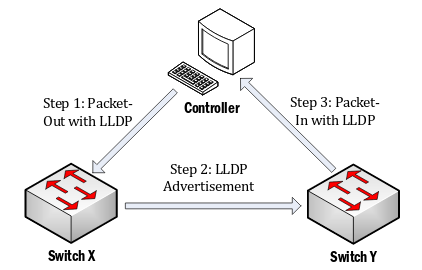
\includegraphics[width=0.6\textwidth]{lldp.png}
  	\caption{Mécanisme de découverte de topologie par envoi de paquets LLDP}
\end{figure}

Au sein du contrôleur même, on trouve tout le logiciel nécessaire pour lier les informations reçues depuis les différentes entités du réseau aux intentions de plus haut niveau émises. Comme sur un système d'exploitation classique, on peut trouver une abstraction plus ou moins riche : selon la maturité du contrôleur et le dynamisme de la communauté qui le porte, on trouvera ainsi de nombreuses différences dans la quantité de développement à fournir pour arriver à un même résultat. Par exemple sur ONOS il est possible de spécifier uniquement une intention de haut niveau qui sera automatiquement traduites en règles qui seront si c'est possible envoyées aux switchs.\\

Le contrôleur offre finalement une API plus ou moins fournie qui permet aux utilisateurs d'écrire des applications en disposant d'abstractions susceptibles de lui éviter l'écriture de code fastidieux.\\

Parmi les contrôleurs SDN les plus connus, on trouve notamment NOX (premier contrôleur SDN, 2008, rendu open source depuis), POX (juin 2011, en python), OpenDayLight (avril 2013, open source, crée par The Linux Foundation), ONOS (l'objet final de ce stage, décembre 2014, open source, développement repris par The Linux Foundation en 2015), et bien d'autres (Beacon, RoseMary, Ryu ...). Certains projets se ressemblent énormément au niveau des choix effectués (langages utilisés, paradigmes ...). Par exemple OpenDayLight et ONOS sont deux contrôleurs très proches dans ce qu'ils offrent (java, architecture OSGi, sécurité vue comme un élément crucial, ...).